\documentclass{article}
\usepackage{nips15submit_e,times}
\nipsfinalcopy
\usepackage[utf8]{inputenc}
\usepackage[T1]{fontenc}
\usepackage{amsmath,amssymb}
\usepackage{graphicx}
\usepackage{booktabs}
\usepackage{multirow}
\usepackage{xcolor}
\usepackage{algorithm}
\usepackage[noend]{algpseudocode}
\usepackage{tikz}
\usetikzlibrary{positioning,arrows.meta,fit}
\usepackage[numbers,sort&compress]{natbib}
\usepackage[colorlinks=true,linkcolor=blue!50!black,citecolor=blue!50!black,urlcolor=blue!50!black]{hyperref}
\usepackage{microtype}

\newcommand{\E}{\mathbb{E}}
\newcommand{\R}{\mathbb{R}}
\newcommand{\todo}[1]{\textcolor{red}{[#1]}}
\newcommand{\inprog}[1]{\textcolor{orange!70!black}{[In progress: #1]}}

\title{Does the Optimizer Change the In-Context Algorithm?\\SGD, AdamW and Muon on Anisotropic Linear Regression}

\author{
Jonah Cha \quad Kevin Chu \quad Ethan Dao \quad Isabella Hu\\
University of California, Berkeley\\
CS 182 final project
}

\begin{document}
\maketitle

\begin{abstract}
Prior work explains how in-context learning (ICL) emerges through data and architecture, but rarely through the optimizer. We train transformers with SGD, AdamW and Muon on in-context linear regression whose inputs vary much more in some directions than others, and compare them at equal in-distribution error early in training. In one-layer linear attention, SGD, Adam and unflattened Muon learn the input directions one at a time, like principal component regression (PCR), while Muon spreads its gain over the weak directions, like ridge regression; flattening the update spectrum by degrees moves the predictor between the two. In GPT-2 models of Garg et al.'s size every optimizer shows a PCR-like cutoff at the same place, but Muon's is softer: in all five seeds its predictions are farther than AdamW's from PCR, without being closer to ridge. Out of distribution, Muon pays a consistent but tiny cost on queries shifted toward high-variance directions and gains at most 6\% on queries shifted toward low-variance ones. Unflattened Muon behaves like AdamW, but SGD matches Muon on how much of the weak directions it has learned. Early in training, the optimizer changes by degree which in-context predictor is reached at a given error, not only how fast.
\end{abstract}

\section{Introduction}
\label{sec:intro}

Transformers trained on prompts of input--output pairs $(x_i, w^\top x_i)$ learn to predict the output for a new input nearly as well as least squares, for linear functions $w$ never seen in training \citep{garg2022}. How they get there may depend on the optimizer, a factor prior work has rarely varied. Consider multi-head linear attention with separate rank-one key and query weights, trained by gradient flow from small initialization. It learns the input directions one at a time, from high to low variance, so a model stopped early approximately implements principal component regression (PCR) on a growing set of directions \citep{zhang2025training}. PCR uses the top $m$ directions fully and ignores the rest; ridge regression uses every direction, shrinking the weak ones more. Muon \citep{jordan2024muon} replaces each weight update by an approximation of its nearest orthogonal matrix, so that all of the update's singular directions move at nearly the same rate. Analyses of simplified Muon find that it learns all directions at the same rate \citep{vasudeva2025,dragutinovic2026}. If that carries over to full transformers, the optimizer would change not only how fast in-context learning emerges but also which in-context algorithm the model runs on the way.

We test this on in-context linear regression with a strongly skewed input spectrum, training the same GPT-2 with SGD, AdamW and Muon. Muon trains about three times faster, so we compare optimizers at equal in-distribution error, not at equal steps. Our key questions and hypotheses are those of our project proposal (Appendix~\ref{app:proposal} lists what else changed):
\begin{enumerate}\setlength{\itemsep}{1pt}
\item Does the optimizer change which in-context algorithm the model runs, when SGD, AdamW and Muon are compared at the same in-distribution error?
\item When does Muon generalize better than AdamW or SGD: when test prompts vary more along directions that had low variance during training, along directions that had high variance, or both?
\item Is flattening the update's singular values, the defining step of Muon, what causes these differences?
\end{enumerate}
\begin{itemize}\setlength{\itemsep}{1pt}
\item[\textbf{H1.}] SGD and AdamW will pass through PCR on a growing set of directions, Muon through a ridge-like estimator that uses every direction partially. All optimizers should end near least squares, as in \citet{garg2022}, but differences should appear along the way: at the same in-distribution error, Muon will have learned more of the low-variance directions.
\item[\textbf{H2.}] Muon will show a smaller error increase than SGD and AdamW when queries emphasize previously low-variance directions, because it learns to use these directions more fully, but a larger one when queries emphasize previously high-variance directions.
\item[\textbf{H3.}] Raising the singular values of Muon's update to a power $p$, from $p=1$ (the update's own spectrum) to $p=0$ (fully flat), will move the learned predictor from PCR toward ridge regression and strengthen both effects in H2.
\end{itemize}
We test all three early in training (at most 4,000 steps), so the end point in H1 is not tested.
\textbf{Contributions.} (i) A paired comparison of SGD, AdamW and Muon at matched in-distribution error in three settings: Garg et al.'s model size (five seeds), a smaller GPT-2 and one-layer linear attention with exact losses. (ii) Three read-outs of the learned predictor (a per-direction probe, the nearest reference estimator and the error under query shifts), with the observation that the probe's negative values are the signature of PCR. (iii) An ablation with a knob from normalized momentum SGD ($p=1$) to Muon ($p=0$).

\section{Related work}
\label{sec:related}
\todo{Related work: being written.}


\section{Methods}
\label{sec:methods}

\subsection{Task}
Each prompt is a sequence $(x_1, y_1, \dots, x_n, y_n, x_q)$ with $n = 40$ examples and a query, $x_i, x_q \in \R^d$ with $d=20$, and $y_i = w^\top x_i$. A fresh task $w \sim \mathcal{N}(0, I_d)$ is drawn for every prompt and inputs are drawn from $\mathcal{N}(0,\Lambda)$ with
\begin{equation}
\Lambda = \mathrm{diag}(\lambda_1,\dots,\lambda_d), \qquad \lambda_j \propto 1/j^2, \qquad \textstyle\sum_j \lambda_j = d .
\end{equation}
The principal directions are the coordinate axes $u_j = e_j$; the variance ratio between the strongest and weakest is $400$, and the top two directions carry 78\% of the total. The outputs are noiseless, so least squares is exact once $n \ge d$. We measure error by
\begin{equation}
\mathrm{err} = \tfrac{1}{d}\,\E\big[(\hat y - y)^2\big],
\label{eq:err}
\end{equation}
which equals $\mathrm{tr}\,\Lambda/d = 1$ for the predictor $\hat y = 0$. Unless stated otherwise, ``error'' is this quantity for the prediction made after all 40 examples, on 1,000 held-out prompts drawn once from a fixed seed. We train on $\mathcal L = \frac{1}{41B}\sum_{b=1}^{B}\sum_{i=1}^{41}(\hat y_{b,i} - y_{b,i})^2$, the squared error of every prediction ($\hat y_{b,i}$ uses the $i-1$ earlier examples; $i = 41$ is the query) over a batch of $B = 64$ prompts, without the $1/d$ of Eq.~\eqref{eq:err}. Training prompts are fresh at every step, so $\mathcal L$ is an unbiased estimate of the population loss.

\subsection{Models}
\textbf{GPT-2.} We use the decoder-only GPT-2 of \citet{garg2022}: 12 layers, 8 heads, width 256, pre-LayerNorm blocks, learned positional embeddings, a $4\times$ GELU MLP and no dropout, with a linear read-in from $\R^{d+1}$ and a linear read-out to a scalar (9.5M parameters). Figure~\ref{fig:setup} shows the input layout. Each example becomes two tokens, $[x_i, 0]$ and $[x_i, y_i]$. Causal attention lets the model predict $y_i$ at token $[x_i, 0]$ from the $i-1$ earlier examples, so one forward pass yields predictions after $0, 1, \dots, 40$ examples. In \citet{garg2022} the $y$ token does not carry $x_i$; with our layout one attention step can read a whole $(x_i, y_i)$ pair, as in the linear-attention constructions of \citet{vonoswald2023} and \citet{ahn2023}. Every hidden weight matrix ($Q, K, V, O$ and both MLP matrices) is initialized from $\mathcal{N}(0, 0.031^2)$, i.e.\ $0.5/\sqrt{256}$, where GPT-2 uses $0.02$ (and $0.02/\sqrt{24} \approx 0.004$ for $O$ and the MLP output). The other initializations are in Table~\ref{tab:hparams}. We changed the layout and the initialization because SGD did not leave the initial loss plateau in our first small GPT-2 with Garg et al.'s.

\begin{figure}[!t]
\centering
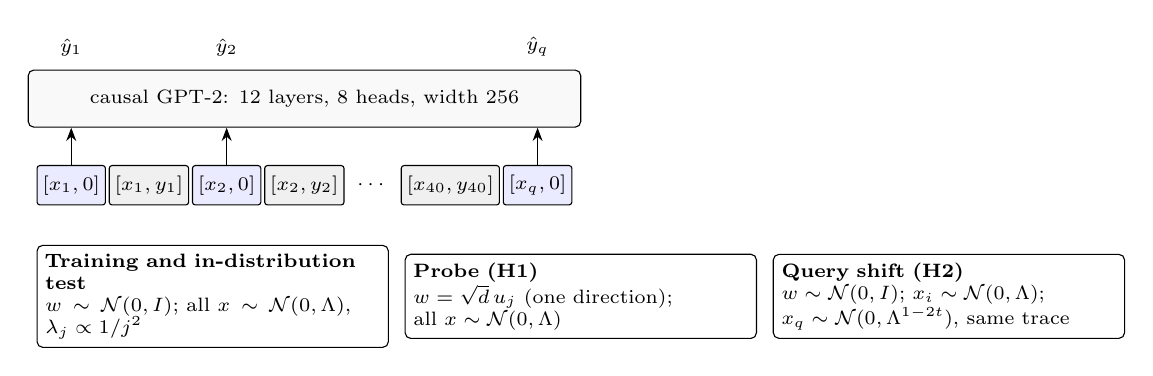
\begin{tikzpicture}[
  tok/.style={draw, rounded corners=1pt, minimum height=5mm, inner sep=2pt, font=\scriptsize},
  qt/.style={tok, fill=blue!8}, ct/.style={tok, fill=gray!12},
  box/.style={draw, rounded corners=2pt, align=left, font=\scriptsize, inner sep=3pt, text width=4.25cm},
  >=Stealth]
\node[qt] (a1) {$[x_1,0]$};
\node[ct, right=1pt of a1] (b1) {$[x_1,y_1]$};
\node[qt, right=1pt of b1] (a2) {$[x_2,0]$};
\node[ct, right=1pt of a2] (b2) {$[x_2,y_2]$};
\node[font=\scriptsize, right=1pt of b2] (dots) {$\cdots$};
\node[ct, right=1pt of dots] (bn) {$[x_{40},y_{40}]$};
\node[qt, right=1pt of bn] (aq) {$[x_q,0]$};
\node[draw, fill=gray!5, rounded corners=2pt, fit=(a1)(aq), inner sep=3pt, yshift=11mm, minimum height=6mm,
      font=\scriptsize, label={[font=\scriptsize]center:causal GPT-2: 12 layers, 8 heads, width 256}] (gpt) {};
\foreach \t/\lab in {a1/{$\hat y_1$}, a2/{$\hat y_2$}, aq/{$\hat y_q$}} {
  \draw[->] (\t.north) -- (\t.north |- gpt.south);
  \node[font=\scriptsize, above=0.5mm of \t.north |- gpt.north] {\lab};
}
\node[box, below=5mm of a1.south west, anchor=north west] (train) {\textbf{Training and in-distribution test}\\ $w\sim\mathcal N(0,I)$; all $x\sim\mathcal N(0,\Lambda)$, $\lambda_j\propto 1/j^2$};
\node[box, right=2mm of train] (probe) {\textbf{Probe (H1)}\\ $w=\sqrt d\,u_j$ (one direction);\\ all $x\sim\mathcal N(0,\Lambda)$};
\node[box, right=2mm of probe] (shift) {\textbf{Query shift (H2)}\\ $w\sim\mathcal N(0,I)$; $x_i\sim\mathcal N(0,\Lambda)$;\\ $x_q\sim\mathcal N(0,\Lambda^{1-2t})$, same trace};
\end{tikzpicture}
\caption{\textbf{Input layout and the three kinds of prompts.} Each example $i$ becomes a query token $[x_i,0]$ (blue), where $y_i$ is predicted, and a context token $[x_i,y_i]$ (grey). The probe changes only the task, so the answer depends on direction $j$ alone; the query shift changes only the query's input distribution ($t>0$: toward low-variance directions, $t<0$: toward high-variance ones).}
\label{fig:setup}
\end{figure}

\textbf{Smaller models.} A smaller GPT-2 (4 layers, 4 heads, width 128, $d = 8$, 32 examples; Appendix~\ref{app:small}), and a one-layer, 8-head linear-attention model with separate rank-one key and query weights \citep{zhang2025training}, $d = 8$, $N = 32$ examples. With $\beta = \frac1N\sum_n y_n x_n$, it predicts
\begin{equation}
\hat y = \beta^\top \Gamma\, x_q, \qquad \Gamma = \textstyle\sum_{h=1}^{8} v_h\, k_h q_h^\top ,
\end{equation}
with $k_h, q_h \in \R^d$ and $v_h \in \R$, and is trained on the squared error of the query. Its population loss $L$, and its loss on any shifted query distribution, can be computed exactly from $\Gamma$ (Appendix~\ref{app:small}). In the principal basis its gain on direction $j$ is $\rho_j = \lambda_j \Gamma_{jj}$, and the best gain at finite $N$ is $\rho_j^\star = \lambda_j N / ((N+1)\lambda_j + \mathrm{tr}\,\Lambda)$ \citep{zhang2025training}. We report $\rho_j/\rho_j^\star$, the fraction of the optimal gain learned, and measure progress by the excess loss $(L - L^\star)/(1 - L^\star)$, where $L^\star$ is the loss at $\rho = \rho^\star$.

\subsection{Optimizers}
For a weight matrix $W \in \R^{m\times n}$ ($m$ output features) with stochastic gradient $G$ of $\mathcal L$:

\textbf{SGD} with heavy-ball momentum in PyTorch's form, $B \leftarrow 0.9B + G$, $W \leftarrow W - \eta B$, after clipping the global gradient norm of all parameters at 1. \textbf{AdamW} \citep{kingma2015adam,loshchilov2019} with $\beta = (0.9, 0.999)$, $\epsilon = 10^{-8}$ and weight decay 0 (that is, Adam). \textbf{Muon} \citep{jordan2024muon} keeps a momentum buffer and replaces the update by an approximation of its polar factor, the orthogonal matrix nearest to it (Algorithm~\ref{alg:muon}). If $M = U S V^\top$ is a singular value decomposition, the polar factor is $UV^\top$: every singular value is set to one, so every singular direction of the update moves by the same amount. Muon approximates it without an SVD by five iterations of an odd quintic polynomial tuned for speed rather than convergence. After Frobenius normalization, singular values above about $3\cdot10^{-3}$ end in $[0.68, 1.20]$, while smaller ones are only multiplied by $a^5 \approx 485$, so directions with a tiny share of the update are not fully flattened. We apply Muon to every weight matrix inside the transformer blocks ($Q$, $K$, $V$, $O$ and both MLP matrices; 99.3\% of the parameters). $Q$, $K$ and $V$ are separate $256\times256$ matrices, each orthogonalized whole, and Newton--Schulz runs in float32. As is standard \citep{jordan2024muon}, AdamW at learning rate $10^{-3}$ trains the rest (read-in, read-out, positional embeddings, LayerNorm gains, biases).

\begin{algorithm}[t]
\caption{Muon update for one weight matrix $W \in \R^{m\times n}$ (our implementation, after \citet{jordan2024muon})}
\label{alg:muon}
\begin{algorithmic}[1]
\Require gradient $G$ of $\mathcal L$ w.r.t.\ $W$; buffer $B$ (initially 0); learning rate $\eta$ (including warm-up)
\State $B \gets \mu B + (1-\mu)\, G$ \Comment{momentum buffer, $\mu = 0.95$}
\State $M \gets (1-\mu)\,G + \mu B$ \Comment{Nesterov look-ahead}
\State $X \gets M / (\|M\|_F + 10^{-7})$; \textbf{if} $m > n$: $X \gets X^\top$
\For{$k = 1,\dots,5$} \Comment{Newton--Schulz: $X \to$ approx.\ $UV^\top$}
  \State $A \gets X X^\top$; \quad $X \gets aX + (bA + cA^2)X$ \Comment{$(a,b,c) = (3.4445, -4.7750, 2.0315)$}
\EndFor
\State \textbf{if} $m > n$: $X \gets X^\top$
\State $W \gets W - \eta\,\sqrt{\max(1, m/n)}\; X$
\end{algorithmic}
\end{algorithm}

\textbf{Spectral knob.} To test whether flattening the singular values is what matters (H3), we replace lines 3--7 of Algorithm~\ref{alg:muon} by an exact SVD of $M$ that keeps a power of its singular values,
\begin{equation}
M = U S V^\top \;\longmapsto\; \sqrt{\min(m,n)}\; \frac{U S^{p} V^\top}{\|U S^{p} V^\top\|_F} ,
\label{eq:knob}
\end{equation}
rescaled to the Frobenius norm of an $m\times n$ orthogonal matrix; momentum and the factor $\sqrt{\max(1, m/n)}$ are unchanged. At $p = 1$ this is momentum SGD with a per-matrix normalized step; at $p = 0$ it is the exact polar factor (at Garg scale $UV^\top$ from a float64 SVD). In between it is steepest descent under the Schatten-$q$ norm with $q = 1+1/p$ \citep{dong2026muonp}: the step $\Delta$ maximizing $\langle M, \Delta\rangle$ subject to $\|\Delta\| \le \eta$, where the Schatten-$q$ norm is the $\ell_q$ norm of the singular values ($q=2$: Frobenius; $q=\infty$: spectral \citep{bernstein2024old}), is proportional to $US^{1/(q-1)}V^\top = US^pV^\top$. We run $p \in \{1, 0.75, 0.5, 0.25, 0.1, 0\}$ in linear attention, $p \in \{1, 0.25, 0\}$ in the small GPT-2 and $p\in\{1, 0\}$ plus standard Muon at Garg scale \inprog{$p = 0.25$ at Garg scale}.

\subsection{Measurements}
\label{sec:measure}
\textbf{Matched error.} Each run is evaluated every 50 steps up to step 2,000 and every 100 after, and read at the first evaluation where its error reaches $0.04$ (primary), $0.05$ or $0.03$ (secondary). Comparing at equal error rather than equal steps removes the speed difference: what remains is \emph{how} the error is distributed.

\textbf{Probe score (H1).} For direction $j$ we build 64 probe prompts with task $w = \sqrt{d}\,u_j$ (so $\|w\|^2 = d$, the typical norm) and inputs drawn as in training, so the correct answer $y = \sqrt d\, x_j$ depends on direction $j$ only. At each prefix length $k$ we compute $\mathrm{relerr}_{j,k} = \sum (\hat y - y)^2 / \sum y^2$ over these prompts, and define the probe score $f_j = 1 - \frac{1}{25}\sum_{k=16}^{40}\mathrm{relerr}_{j,k}$. $f_j = 1$ is perfect and $f_j = 0$ is no better than predicting zero, but $f_j$ has no lower bound. An estimator that ignores direction $j$ still fits the probe's $y$ with the directions it uses, so its predictions are noise and $f_j < 0$. On these prompts PCR$_m$ (below) gives $f_j \ge 0.87$ for $j \le m$ and $-0.4$ to $-0.9$ for $j > m$, while ridge ($\alpha = 0.1$ to 100) never goes below $-0.02$ (Figure~\ref{fig:h1}a, grey). We summarize the weak directions by the probe score $\bar f$, the mean of $f_j$ over $j = 3,\dots,20$ (every arm learns directions 1--2, 78\% of the variance, before error 0.1), and by the bounded score $\bar f_+$, the mean of $\max(f_j, 0)$, which counts only what has been learned.

\textbf{Which algorithm (H1).} We compare the model's predictions on the held-out prompts with two families of reference estimators computed from the same context $(X, y)$:
\begin{align}
\text{ridge:}\quad \hat y &= x_q^\top (X^\top X + \alpha I)^{-1} X^\top y, \qquad \alpha \in \{10^{-3}, 3\cdot 10^{-3}, \dots, 100\},\\
\text{PCR}_m:\quad \hat y &= (U_m^\top x_q)^\top (Z^\top Z + s_m I)^{-1} Z^\top y, \qquad Z = X U_m,\; s_m = \textstyle\sum_{j>m}\lambda_j,
\end{align}
where $U_m$ holds the top $m$ population directions, $m = 1,\dots,20$. PCR$_m$ is ridge restricted to the top $m$ directions, treating the omitted ones as noise of variance $s_m$ (plain least squares in the subspace diverges when the number of examples is near $m$); PCR$_d$ is least squares (pseudo-inverse). For each evaluation we take the mean squared distance between the model's predictions and each reference's over predictions with 8--40 examples, pick the nearest PCR and ridge references, and report both distances and their ratio (above 1: closer to ridge).

In linear attention we fit a PCR step and a ridge shrinkage curve directly to the gain profile $\rho_j/\rho_j^\star$, average the two residuals over matched excess-loss levels from 0.5 to 0.1, and report their ratio per seed (Appendix~\ref{app:small}).

\textbf{Query shift (H2).} We keep the task and the context examples and draw only the query from $\mathcal{N}(0, \Lambda^{1-2t})$, rescaled to trace $d$, for $t \in \{-1, -0.5, 0, 0.25, 0.5, 0.75, 1\}$ (256 prompts, every 100 steps). $t=0$ is the training distribution; $t>0$ moves the query toward low-variance directions (``rare-ward''; $t=0.5$ is isotropic, $t=1$ inverts the spectrum) and $t<0$ toward high-variance ones (``common-ward''). Each run is read where its own unshifted error on these prompts (in the units of Eq.~\eqref{eq:err}) crosses the matched level, interpolating log error between evaluations. Arms are then matched exactly on the same prompts, so comparing shifted errors compares error increases; with fewer prompts than in H1, this read can fall a few hundred steps from the H1 read. We report each arm's shifted error divided by AdamW's in the same seed, and the geometric mean of these ratios over $t<0$ or $t>0$.

\textbf{Error bars and statistics.} Bars and bands at Garg scale are $\pm1$ sample s.d.\ over five training seeds, which vary the initialization and the data order; the evaluation prompts are fixed. For the three-seed linear-attention runs we show medians and min--max ranges, since a standard deviation of three values is unreliable. Comparisons are paired by seed (same initialization and data stream). Our main statistic is the number of seeds in which the difference has the predicted sign, with an exact one-sided sign test (5/5 gives $p = 1/32 = 0.031$, the smallest possible; 4/5 gives $0.19$); one-sided paired $t$-tests (4 d.f.) are given as $p_t$. The error levels are read from the same runs, and we do not correct for multiple comparisons.

\subsection{Hyperparameters and controls}
\label{sec:controls}

Table~\ref{tab:hparams} (Appendix~\ref{app:lr}) lists every setting at Garg scale with its source and the reason for it, and Table~\ref{tab:smallhp} (Appendix~\ref{app:small}) does the same for the smaller settings and the measurements. In brief: batch 64, 100 warm-up steps then a constant rate, no curriculum, at most 4,000 steps, seeds 10--14; SGD at learning rate 0.1, AdamW at $3\cdot10^{-4}$, Muon at 0.007 and Muon with $p=1$ at $5\cdot10^{-4}$. Within a setting only the optimizer and its learning rate change: for a given seed, all arms share the initialization, the training prompts and their order, and the evaluation prompts. The Muon arms also train the non-matrix parameters (0.7\%) with AdamW at $10^{-3}$ and stop earlier; the $p=1$ arm shares both, so neither explains a difference between Muon and $p=1$. A one-seed check at Garg scale found no learning rate about $3\times$ lower or higher with more than 1.5\% lower training loss (Appendix~\ref{app:lr}). Absolute numbers are not comparable with \citet{garg2022}, whose spectrum, layout, initialization, curriculum and training length differ. Across our three settings the architecture, $d$ and $N$, the batch size (1,024 versus 64), SGD itself (plain gradient descent versus momentum with clipping) and the matched quantity all change at once, so we compare settings only qualitatively.


\section{Results}
\label{sec:results}

\begin{table}[t]
\caption{\textbf{Results in three settings.} ``Common-ward'' and ``rare-ward'': queries shifted toward high- and low-variance directions. Linear-attention levels are excess loss; the residual ratio is PCR over ridge (above 1: closer to ridge). Details: Section~\ref{sec:results} and Appendix~\ref{app:small}.}
\label{tab:summary}
\vspace{2pt}
\centering\footnotesize
\setlength{\tabcolsep}{3pt}
\begin{tabular}{@{}p{0.5cm}p{4.4cm}p{3.3cm}p{5.0cm}@{}}
\toprule
 & Linear attention (3 seeds) & Small GPT-2 (2 seeds) & Garg-scale GPT-2 (5 seeds, error 0.04) \\
\midrule
H1 & Yes. SGD, Adam, $p \ge 0.25$: PCR-like step after 2--3 directions (0.22--0.92); Muon, $p \le 0.1$: ridge-like (1.65--3.19) & Partly. Weakest direction at error 0.03: 0.61 Muon, 0.50 SGD, 0.39 AdamW; all arms closer to ridge & Partly. Same PCR-like cutoff for all; Muon's is softer: $\bar f$ $+0.08$ vs AdamW (5/5), $\bar f_+$ $+0.02$ (4/5), none vs SGD; farther from PCR, not closer to ridge \\
\addlinespace
H2 & At excess loss 0.1 vs Adam: $1.28$--$1.39\times$ common-ward, $0.92$--$0.95\times$ rare-ward & One seed: vs AdamW 4--36\% higher common-ward, 2--31\% lower rare-ward & Vs AdamW: common-ward $1.3$--$1.8\times$ (5/5) but $+0.004$ absolute; rare-ward at most 6\% lower (4/5). Vs SGD: same signs in 4/5, rare-ward at most 7\% \\
\addlinespace
H3 & Yes: PCR-like to ridge-like between $p = 0.25$ and $0.1$; mean gain on directions 3--8 from 0.03 ($p=1$) to 0.20 ($p=0$) & One seed, untuned: $\bar f$ 0.72, 0.82, 0.83 at $p=1, 0.25, 0$; no trend in PCR/ridge & Ends only: $p=1$ matches AdamW on every measure, $p=0$ (1 seed) matches Muon; but SGD matches Muon on $\bar f_+$ \\
\bottomrule
\end{tabular}
\end{table}

\subsection{Training and validation loss}
In Figure~\ref{fig:loss}a the logged training loss (the mean over the steps since the previous evaluation) lags the validation loss early in training and otherwise matches it, as expected when every training prompt is new. Figure~\ref{fig:loss}b shows the quantity we match on. Muon reaches error 0.04 at steps 550--650, against 1,750--2,300 for AdamW, 1,450--2,000 for Muon with $p=1$ and 3,300--3,900 for SGD. Its lead over AdamW grows from about $2\times$ at error 0.1 to $3.6$--$4.2\times$ at 0.03. Scales are logarithmic because the curves span more than an order of magnitude.

\begin{figure}[t]
\centering
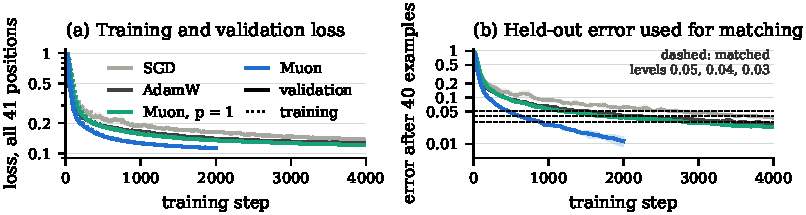
\includegraphics[width=\linewidth]{figures/fig_loss.pdf}
\caption{\textbf{Training and validation loss at Garg scale.} (a) Squared error$/d$ over all 41 positions: validation (solid, 1,000 held-out prompts) and training (dotted, mean since the previous evaluation). (b) Held-out error after 40 examples (Eq.~\ref{eq:err}), used for matching. Mean over seeds 10--14, bands $\pm 1$ s.d.; log scales; Muon to step 2,000, where all five seeds exist.}
\label{fig:loss}
\end{figure}

\subsection{H1: every optimizer is PCR-like on the probe; Muon's cutoff is softer}
\label{sec:h1}

Figure~\ref{fig:h1}a shows the probe profile at error 0.04. Every arm has learned directions 1--11 about equally well and, beyond a cutoff, gives the strongly negative scores that PCR gives on the directions it omits; no arm looks like ridge, whose score falls smoothly and stays non-negative. At each error all arms have the same number of directions with $f_j > 0.5$: 9--10 at 0.05, 10--12 at 0.04, 12--13 at 0.03. The optimizers differ at the cutoff. AdamW drops from 0.54 at direction 11 to $-0.59$ at direction 13, and unflattened Muon almost identically. SGD's drop comes one direction later. Muon's drop is spread over directions 12--15 (0.45, 0.27, $-0.24$, $-0.47$).

On the probe score $\bar f$ (Table~\ref{tab:h1}, Figure~\ref{fig:h1}b) Muon leads AdamW by $+0.07$ to $+0.08$ in every seed at every level from 0.05 to 0.03 (5/5, sign test $p=0.031$), but mostly by being less negative beyond the cutoff, not by learning more. On the bounded score $\bar f_+$ the lead shrinks to $+0.020$ at error 0.04 (4/5 seeds; $p_t = 0.028$), $+0.029$ at 0.05 (5/5) and $+0.009$ at 0.03 (3/5). Against SGD the raw lead is $+0.04$ (5/5) and the bounded lead vanishes ($+0.004$, 3/5). Muon leads unflattened Muon in every seed, by $+0.065$ raw and $+0.026$ bounded. At error 0.1 every arm has learned only the first six to eight directions.

\begin{figure}[t]
\centering
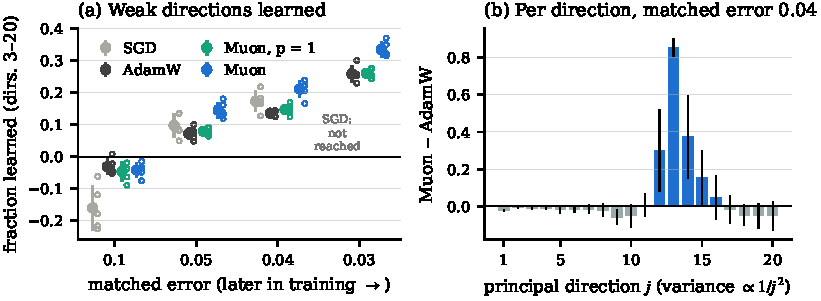
\includegraphics[width=\linewidth]{figures/fig_h1.pdf}
\caption{\textbf{H1 at Garg scale, error 0.04.} (a) Probe score per direction, mean over seeds 10--14, bands $\pm1$ s.d.\ ($p=1$: thin line). Grey: the probe applied to the nearest references, PCR$_{11}$ (dashed) and ridge with $\alpha = 1$ (dash-dotted). (b) Paired differences between Muon and each arm in $\bar f$ (filled) and $\bar f_+$ (open); mean $\pm1$ s.d., circles: seeds.}
\label{fig:h1}
\end{figure}

\begin{table}[t]
\caption{\textbf{H1 at Garg scale, error 0.04} (per-seed values and errors 0.05 and 0.03 in Appendix~\ref{app:seeds}). Dirs.: number of directions with $f_j > 0.5$, range over seeds. $\bar f$, $\bar f_+$: mean $\pm$ s.d.\ over seeds 10--14. Distances: mean squared distance to the nearest PCR and ridge reference, mean over seeds (least squares: 0.049); ratio: their quotient, range over seeds (number of seeds above 1). Difference rows: mean paired difference (seeds with the sign shown; tests in Table~\ref{tab:seeds}).}
\label{tab:h1}
\vspace{2pt}
\centering\footnotesize
\setlength{\tabcolsep}{4pt}
\begin{tabular}{@{}lcccccc@{}}
\toprule
 & Dirs. & Probe $\bar f$ & Bounded $\bar f_+$ & PCR dist. & Ridge dist. & Ratio \\
\midrule
SGD & 11--12 & $0.17 \pm 0.03$ & $0.449 \pm 0.011$ & 0.023 & 0.021 & 0.89--1.29 (4) \\
AdamW & 10--11 & $0.14 \pm 0.01$ & $0.433 \pm 0.008$ & 0.019 & 0.021 & 0.79--0.97 (0) \\
Muon & 11--12 & $0.21 \pm 0.03$ & $0.453 \pm 0.011$ & 0.026 & 0.022 & 1.11--1.20 (5) \\
Muon, $p=1$ & 10--11 & $0.15 \pm 0.02$ & $0.426 \pm 0.016$ & 0.019 & 0.020 & 0.82--1.03 (1) \\
\midrule
Muon $-$ AdamW & & $+0.076$ (5/5) & $+0.020$ (4/5) & $+0.007$ (5/5) & $+0.002$ (5/5) & \\
Muon $-$ SGD & & $+0.038$ (5/5) & $+0.004$ (3/5) & $+0.003$ (4/5) & $+0.001$ (4/5) & \\
Muon $-$ ($p{=}1$) & & $+0.065$ (5/5) & $+0.026$ (5/5) & $+0.007$ (5/5) & $+0.002$ (4/5) & \\
\bottomrule
\end{tabular}
\end{table}

The reference estimators tell the same story (Table~\ref{tab:h1}). Muon's predictions are farther than AdamW's from the nearest PCR reference in every seed (15/15 seed $\times$ error pairs at 0.05--0.03), but not closer to ridge: they are also slightly farther from the nearest ridge reference (5/5 at 0.04). Their PCR/ridge ratio is above 1 because Muon moves away from PCR, not toward ridge, and neither family fits any model closely (the nearest reference is about half as far as least squares). SGD again sits nearer Muon than AdamW, and at error 0.1 SGD, AdamW and Muon are all closer to ridge in every seed. In short, H1 holds against AdamW only as a difference of degree, a softer cutoff, and not against SGD.

\subsection{H2: a consistent but tiny common-ward cost and a small rare-ward gain}

Figure~\ref{fig:h2} shows the query-shift test at error 0.04. Muon's error exceeds AdamW's on common-ward queries in every seed (geometric mean over $t<0$: $1.28$--$1.81\times$; 5/5 at each of errors 0.05, 0.04 and 0.03). On rare-ward queries it is lower in four of five seeds at errors 0.04 ($0.96$--$1.03\times$) and 0.03, but in three of five at 0.05 ($0.98$--$1.01\times$). The ratios hide that the two effects differ in size (Figure~\ref{fig:h2}b): AdamW's error at $t=-1$ is only 0.007, so Muon's cost there is $+0.004$, while its gain at $t=+1$ is $-0.028$ on an error of 0.83. Still, at $t=+1$ every model's error is 0.81--0.88 of predicting zero, because no arm has learned directions 14--20. Removing the flattening removes both effects ($p=1$: cost in 1/5 seeds, gain in 2/5). Against SGD, Muon's error is higher at $t=-1$ and lower at $t=+1$ in 4/5 seeds each, by at most 7\% at $t=+1$.

\begin{figure}[t]
\centering
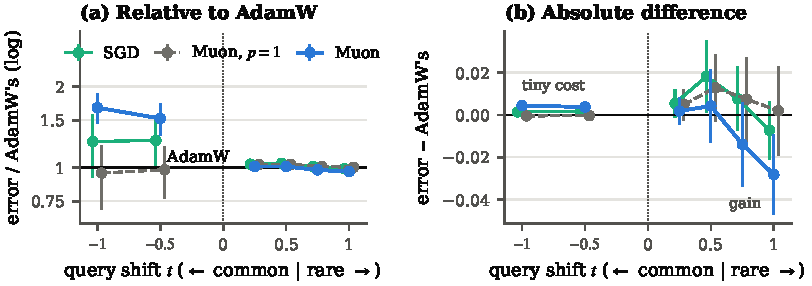
\includegraphics[width=\linewidth]{figures/fig_h2.pdf}
\caption{\textbf{H2 at Garg scale, error 0.04.} (a) Shifted-query error divided by AdamW's in the same seed (log scale: a cost and a gain by the same factor look the same size). (b) The difference. Mean over seeds 10--14, bars $\pm1$ s.d.; $t<0$: query toward high-variance directions. AdamW's errors at $t = -1, -0.5, 0.25, 0.5, 0.75, 1$: 0.007, 0.007, 0.19, 0.49, 0.70, 0.83.}
\label{fig:h2}
\end{figure}

\subsection{H3: removing the flattening removes the effect}

At Garg scale only the ends of the knob have been run. Muon without flattening ($p=1$) is indistinguishable from AdamW on every measure above, and most of its speed-up is gone. Exact orthogonalization ($p=0$, seed 10 only) behaves like standard Muon (Appendix~\ref{app:seeds}). Flattening is thus necessary for Muon's differences here, but not the only route to them: SGD, which does not flatten, matches Muon on the bounded score and is also farther from PCR than AdamW.

Linear attention lets us vary $p$ finely (Figure~\ref{fig:linattn}). By excess loss 0.1, SGD, Adam and every $p \ge 0.25$ have learned the two strongest directions and part of the third (a fifth for SGD and $p = 1$, half for Adam): a PCR-like step, with residual ratio 0.22--0.40 for $p \ge 0.25$, 0.34 for SGD and 0.92 for Adam. Below $p = 0.25$ the gain spreads to the weaker directions and the fit becomes ridge-like (1.65 at $p=0.1$, 3.19 at $p=0$); the mean gain on directions 3--8 rises from 0.03 at $p=1$ to 0.20 at $p=0$. The change is concentrated between $p = 0.25$ and 0, not spread evenly over $p$. Standard Newton--Schulz Muon is ridge-like too (2.55), but its gain stops at direction 4, consistent with Newton--Schulz leaving very small singular values unflattened (Section~3.3).

\begin{figure}[t]
\centering
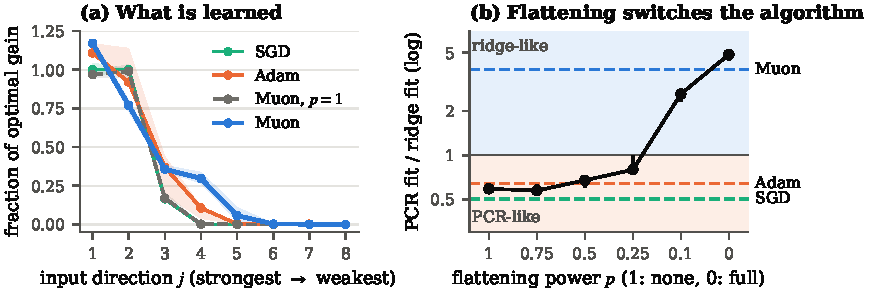
\includegraphics[width=\linewidth]{figures/fig_linattn.pdf}
\caption{\textbf{Linear attention, $\lambda_j \propto 1/j^2$, $d=8$.} (a) Fraction of the optimal gain per direction at excess loss 0.1: median over 3 seeds (SGD: 2 reach 0.1), bands min--max; thin lines $p = 1, 0.25, 0.1$ ($p = 0.75, 0.5$ overlap $p=1$). (b) PCR over ridge residual, averaged over 8 excess-loss levels from 0.5 to 0.1, per $p$ (evenly spaced, not to scale); median, bars and bands min--max; lines: SGD, Adam, standard Muon. Log axis: $k$ times closer to PCR or ridge is the same distance from 1.}
\label{fig:linattn}
\end{figure}

\section{Discussion and conclusion}
\label{sec:discussion}

Within the first 4,000 steps, the optimizer changes which input directions the in-context predictor uses at a given error, not only how fast the error falls: clearly in linear attention, by degree in the GPT-2s. Linear attention matches H1 and H3: gradient methods follow the PCR path, and flattening moves the predictor to a ridge-like shape. In the Garg-scale GPT-2 every optimizer keeps a PCR-like cutoff at the same place; Muon softens it, which shows up out of distribution as a small rare-ward gain and a consistent but tiny common-ward cost. At equal steps, by contrast, Muon is simply further along: at step 2,000 its shifted-query error is 0.26--0.71 of AdamW's for every shift and seed.

Why does SGD group with Muon, and AdamW with unflattened Muon? We have not separated the candidates. AdamW normalizes per weight coordinate \citep{xie2025adam}, and after a random read-in each input direction is spread over many hidden coordinates; the $p=1$ arm normalizes each matrix's update, while SGD's clipping, when active, normalizes all matrices jointly; depth, the nonlinearities and momentum may also matter. Batch-64 noise should act against Muon, pushing its update back toward the gradient and restoring sequential learning \citep{jacobs2026}, which may be one reason Muon differs from AdamW only by degree.

\textbf{Status and limitations.} In progress for the final version: \inprog{the knob at $p = 0.25$ at Garg scale; more seeds for exact orthogonalization (seed 10 only) and for the small-GPT-2 query shift and knob (one seed)}. Everything else is final. Limitations: five seeds give coarse tests; training is short (at most 4,000 steps against Garg et al.'s 500,000), so we cannot say whether every optimizer ends near least squares or whether the differences persist; learning rates were checked at Garg scale with one seed and 1,500 steps, and AdamW's was slightly low (Appendix~\ref{app:lr}); and we test one task and one input spectrum.

\bibliographystyle{plainnat}
\bibliography{refs}

\appendix
\section{Use of generative AI tools}
\label{app:ai}
\todo{TODO: to be written by the team.}

\section{Hyperparameters and learning rates}
\label{app:lr}
\begin{table}[h]
\caption{\textbf{Settings at Garg scale and where they come from.} ``Ours'' marks choices made for this study.}
\label{tab:hparams}
\vspace{2pt}
\centering\footnotesize
\setlength{\tabcolsep}{4pt}
\begin{tabular}{@{}p{2.2cm}p{4.1cm}p{6.4cm}@{}}
\toprule
Setting & Value & Source / reason \\
\midrule
$d$, $n$ & $20$, $40$ & \citet{garg2022}: final curriculum stage for $d=20$ \\
Model & 12 layers, 8 heads, width 256 & \citet{garg2022} \\
Batch & 64 prompts, fresh every step & \citet{garg2022} \\
Input spectrum & $\lambda_j \propto 1/j^2$, $\mathrm{tr}\,\Lambda = d$ & Ours: strongly imbalanced directions \\
Token layout & $[x_i,0]$, $[x_i,y_i]$ & Ours: lets SGD train (Sec.~3.2) \\
Hidden init. & $\mathcal{N}(0, 0.031^2)$ ($0.5/\sqrt{\text{width}}$) for $Q,K,V,O$ and both MLP matrices & Ours: lets SGD train (Sec.~3.2) \\
Other init. & biases 0; read-in $\mathcal N(0, 1/(3(d+1)))$; positions $\mathcal N(0, 0.02^2)$; read-out PyTorch default & Read-in: PyTorch's default variance, but rotation-invariant in distribution \\
Curriculum & none & Ours: identical data for all arms \\
Schedule & 100-step linear warm-up, then constant & Ours: no decay phase coincides with the matched reads, and a run's first $k$ steps equal a $k$-step run (App.~\ref{app:lr}) \\
Steps & 4,000 (Muon 2,000--3,000) & Compute; all arms but SGD reach error 0.03 \\
Seeds & 10--14 & 5 per arm \\
\midrule
SGD & lr 0.1, momentum 0.9, clip 1 & Small-GPT-2 pilot; checked at Garg scale \\
AdamW & lr $3\cdot10^{-4}$, $\beta=(0.9,0.999)$, no decay & Pilot value tuned on isotropic inputs; checked. Weight decay 0: no arm has an explicit regularizer, and weight decay moves which estimator emerges \citep{raventos2023} \\
Muon (matrices) & lr 0.007, momentum 0.95 (Nesterov), 5 NS steps & Small-GPT-2 sweep; \citet{jordan2024muon} \\
Muon (non-matrix) & AdamW, lr $10^{-3}$ & Following \citet{jordan2024muon}; not tuned \\
Muon, $p=1$ & lr $5\cdot10^{-4}$ & Two pilots (0.007 stalled, 0.002 noisy); best of four rates (App.~\ref{app:lr}) \\
\bottomrule
\end{tabular}
\end{table}

\textbf{How the rates were chosen.} Sweeps on the first version of the smaller GPT-2 (seed 0) kept the rate with the lowest area under the error curve on separate selection prompts. AdamW won at $5\times10^{-4}$; Muon's 0.007 tied 0.01 on area and had the lower final error. SGD did not train in that model at any rate, so 0.1 with gradient clipping was carried over; in the redesigned model (Section~3.2) it beat 0.3. These rates were reused at Garg scale, except that AdamW used $3\times10^{-4}$, an earlier pilot value tuned on isotropic inputs. Unflattened Muon ($p=1$) used $5\times10^{-4}$ after 0.007 stalled and 0.002 was noisy. In the linear-attention model every arm had its own six-point sweep on seed 0, selected by mean loss over training (Appendix~\ref{app:small}).

\textbf{Check at Garg scale.} We trained seed 10 for 1,500 steps at rates about $3\times$ below and above each rate used, plus AdamW at $5\times10^{-4}$ (the smaller model's choice), and compared training loss over steps 1,400--1,500 (Table~\ref{tab:lr}). Every training prompt is new, so this estimates the population loss without touching the evaluation prompts; the rates used are read from the main runs at the same steps (the schedule is constant after warm-up, so their first 1,500 steps are identical to a 1,500-step run). The rate used was best for unflattened Muon. Muon's best rate (0.0025) was 0.7\% lower and SGD's (0.03) 0.4\% lower. AdamW's rate was slightly low: $5\times10^{-4}$ and $10^{-3}$ gave 1.5\% and 1.4\% lower loss, but the same error at step 1,500 (0.052--0.053), and first reached error 0.05 only 50 steps sooner (step 1,350 against 1,400). At error 0.05, Muon leads AdamW for every pair of rates that reach that error by step 1,500: its weak-direction fraction is 0.11--0.19 at its three rates, against 0.05--0.07 for AdamW at $3\times10^{-4}$, $5\times10^{-4}$ and $10^{-3}$ (interpolated to exactly 0.05: 0.10--0.14 against 0.06--0.07). AdamW at $10^{-4}$ and every SGD rate stay above error 0.05 through step 1,500, so H1 against SGD, and at lower errors, was not checked.

\begin{table}[h]
\caption{\textbf{Learning-rate check at Garg scale}, seed 10; training loss averaged over steps 1,400--1,500. The rate used in the main runs is in bold. $p=1$ at 0.007 is an earlier run stopped at step 1,500.}
\label{tab:lr}
\centering\small
\begin{tabular}{@{}lll@{}}
\toprule
Optimizer & Learning rates & Training loss \\
\midrule
SGD & 0.03, \textbf{0.1}, 0.3 & 0.1747, \textbf{0.1755}, 0.2092 \\
AdamW & $10^{-4}$, $\mathbf{3\cdot10^{-4}}$, $5\cdot10^{-4}$, $10^{-3}$ & 0.1659, \textbf{0.1501}, 0.1479, 0.1480 \\
Muon & 0.0025, \textbf{0.007}, 0.02 & 0.1160, \textbf{0.1168}, 0.1339 \\
Muon, $p=1$ & $1.5\cdot10^{-4}$, $\mathbf{5\cdot10^{-4}}$, $1.5\cdot10^{-3}$, 0.007 & 0.1571, \textbf{0.1451}, 0.1523, 0.3475 \\
\bottomrule
\end{tabular}
\end{table}


\section{Per-seed and supplementary results}
\label{app:seeds}
Table~\ref{tab:seeds} gives the per-seed paired differences behind Table~\ref{tab:h1}: the weak-direction fraction (directions 3--20) of Muon minus that of the other optimizer in the same seed, with one-sided paired $t$-tests (4 degrees of freedom).

\begin{table}[h]
\caption{\textbf{Per-seed paired differences} in the weak-direction fraction at Garg scale.}
\label{tab:seeds}
\centering\footnotesize
\setlength{\tabcolsep}{4pt}
\begin{tabular}{@{}llrrrrrrr@{}}
\toprule
Error & Comparison & Seed 10 & Seed 11 & Seed 12 & Seed 13 & Seed 14 & Mean & $p$ \\
\midrule
0.05 & Muon $-$ AdamW & $+0.101$ & $+0.048$ & $+0.089$ & $+0.081$ & $+0.050$ & $+0.074$ & 0.001 \\
0.05 & Muon $-$ SGD & $+0.112$ & $+0.038$ & $+0.001$ & $+0.096$ & $-0.005$ & $+0.048$ & 0.057 \\
0.05 & Muon $-$ Muon ($p=1$) & $+0.098$ & $+0.042$ & $+0.046$ & $+0.107$ & $+0.041$ & $+0.067$ & 0.005 \\
0.04 & Muon $-$ AdamW & $+0.063$ & $+0.040$ & $+0.081$ & $+0.114$ & $+0.081$ & $+0.076$ & 0.002 \\
0.04 & Muon $-$ SGD & $+0.079$ & $+0.001$ & $+0.039$ & $+0.065$ & $+0.006$ & $+0.038$ & 0.034 \\
0.04 & Muon $-$ Muon ($p=1$) & $+0.082$ & $+0.021$ & $+0.069$ & $+0.069$ & $+0.083$ & $+0.065$ & 0.002 \\
0.03 & Muon $-$ AdamW & $+0.088$ & $+0.066$ & $+0.069$ & $+0.098$ & $+0.060$ & $+0.076$ & $<0.001$ \\
0.03 & Muon $-$ Muon ($p=1$) & $+0.065$ & $+0.046$ & $+0.114$ & $+0.077$ & $+0.072$ & $+0.075$ & 0.001 \\
\bottomrule
\end{tabular}
\end{table}

Read at exactly each error level (linear interpolation between the two evaluations that bracket the first crossing), the mean differences are: Muon $-$ AdamW $+0.069$, $+0.063$, $+0.086$ at errors 0.05, 0.04, 0.03 (all $p<0.001$); Muon $-$ SGD $+0.058$ ($p=0.024$) and $+0.036$ ($p=0.037$); Muon $-$ ($p=1$) $+0.063$, $+0.048$, $+0.083$ ($p \le 0.006$).


\section{Smaller models and measurement settings}
\label{app:small}
\textbf{Linear attention.} The model of Section~3.2 ($d = 8$, $N = 32$, 8 heads with rank-one keys and queries, weights initialized from $\mathcal N(0, 10^{-4})$) is trained for 4,000 steps on batches of 1,024 fresh prompts with $\lambda_j \propto 1/j^2$. Its population loss and its loss on shifted query distributions are computed exactly from $\Gamma$ every 10 steps. SGD here is plain gradient descent without momentum, as in \citet{zhang2025training}; Adam has no weight decay; Muon and the knob arms update the stacked key and query matrices, with Adam on the head scalars $v_h$. Each arm's learning rate is selected on seed 0 from a six-point grid by mean loss over training, and seeds 1--2 are run at that rate. The grids are $\{0.003, 0.01, 0.02, 0.05, 0.1, 0.2\}$ for SGD, $\{3\cdot10^{-4}, 10^{-3}, 3\cdot10^{-3}, 10^{-2}, 3\cdot10^{-2}, 10^{-1}\}$ for Adam and $\{10^{-3}, 3\cdot10^{-3}, 10^{-2}, 2\cdot10^{-2}, 5\cdot10^{-2}, 10^{-1}\}$ for Muon and every knob arm. The selected rates are 0.02 (SGD), 0.03 (Adam) and 0.02 (standard Muon and every knob arm). Levels are excess loss, $(L - L^\star)/(1 - L^\star)$, where $L^\star$ is the best loss this model can reach. Query shifts use the same $\Lambda^{1-2t}$ family; at excess loss 0.1, standard Muon's error relative to Adam's is 1.39 and 1.28 for the two most common-ward shifts and 0.92 and 0.95 for the two most rare-ward ones (median over seeds); at 0.05 the common-ward ratios are 1.00 and 1.02 and the rare-ward ones 0.96 and 0.97. SGD reaches excess loss 0.1 in two of three seeds and never reaches 0.05.

\textbf{Smaller GPT-2.} 4 layers, 4 heads, width 128, $d = 8$, 32 examples, batch 64, hidden initialization 0.044, the token layout of Section~3.2 and $\lambda_j \propto 1/j^2$. Learning rates: SGD 0.1 with clipping (4,000 steps), AdamW $5\times10^{-4}$ (6,000 steps), Muon 0.007 (3,000 steps), seeds 10 and 11. The knob arms ($p = 1, 0.25, 0$; seed 10) all use Muon's rate 0.007, so $p=1$ is untuned and about eight times slower. Its query-shift test was run for seed 10 only.

\textbf{Interpretation caveat.} The linear-attention profile measures the learned gain $\rho_j/\rho^\star_j$ directly, while the GPT-2 measurements infer it from predictions; the PCR-versus-ridge statistics in the two settings are therefore different measurements of the same idea and should not be compared numerically.


\section{Reproducibility and compute}
\label{app:repro}
Code, job files, training logs and checkpoints are at \url{https://github.com/MERC13/cs182finalproject}. The scripts in \texttt{scripts/} compute every figure and number in this paper from the committed logs (the README lists which script produces what).


\section{Changes since the proposal}
\label{app:proposal}
The key questions and hypotheses in Section~\ref{sec:intro} are those of our revised proposal, unchanged except that H3 names ``the update's own spectrum'' (the knob acts on the momentum, not on the raw gradient). Table~\ref{tab:proposal} lists what else changed.

\begin{table}[h]
\caption{\textbf{Changes since the revised proposal.}}
\label{tab:proposal}
\vspace{2pt}
\centering\footnotesize
\begin{tabular}{@{}p{3.8cm}p{4.5cm}p{4.7cm}@{}}
\toprule
Proposal & This paper & Why \\
\midrule
Main model: 4-layer, width-128 GPT-2, $d = 8$, $N = 32$ (Garg scale as a pilot) & Garg et al.'s 12-layer, width-256 GPT-2 with $d = 20$, $n = 40$; the small model in Appendix~\ref{app:small} & The pilot effects held at the standard testbed size, which makes the results comparable with prior work \\
5 seeds per arm & Garg scale: 5 seeds for SGD, AdamW, Muon and $p=1$; 1 for $p=0$. Linear attention: 3. Small GPT-2: 2 (knob and shift: 1) & CPU budget; the Garg-scale runs took about 70 CPU-hours \\
Knob at $p \in \{1, 0.25, 0\}$ in the GPT-2 & $p \in \{1, 0\}$ and standard Muon at Garg scale; $p = 0.25$ in progress & Each $p$ needs its own learning rate ($p=1$ needed one $14\times$ lower than Muon's) \\
Knob at $p \in \{1, 0.5, 0.25, 0.1, 0\}$ in linear attention & Added $p = 0.75$ & To check the weakly flattened end \\
Own learning-rate sweep per optimizer & Sweeps on the small GPT-2, checked at Garg scale with one seed (Appendix~\ref{app:lr}) & Compute \\
2,000 test prompts & 1,000 held-out prompts, 64 probe prompts per direction, 256 query-shift prompts per shift & Evaluation runs every 50--100 steps \\
``Fraction of each direction learned'' & Probe score $\bar f$ and bounded score $\bar f_+$ & $f_j$ has no lower bound, and its negative values mark PCR (Section~\ref{sec:measure}) \\
Shifts of which tasks appear (linear model) & Not reported & Outside the three hypotheses \\
Compute target: about 25 hours & About 85 CPU-hours at Garg scale, including the learning-rate check & Larger model than planned \\
\bottomrule
\end{tabular}
\end{table}

\textbf{First proposal draft.} Our first draft asked four questions (speed, the effect of the amount of imbalance, generalization to rare-ward queries, and which algorithm). It varied the input covariance ($\lambda_j \propto 1$, $1/j$ or $1/j^2$, aligned or rotated) and compared optimizers at equal steps. Pilots answered the speed question: Muon reaches low error about three times sooner (Section~4.1). They found no effect of rotating the inputs on AdamW in our GPT-2. The revised proposal therefore fixed one aligned $1/j^2$ spectrum, compared optimizers at matched error, and added the knob and the linear-attention model. SGD did not leave the initial plateau in the first small GPT-2 at any setting we tried; the token layout and initialization of Section~3.2 fixed this.


\end{document}
